\documentclass{beamer}
\usepackage[T1]{fontenc}
\usepackage[utf8]{inputenc}
\usepackage[frenchb]{babel}
\usepackage{graphicx}
\usepackage{subfig}
\usepackage{colortbl}
\usepackage{tikz}
\usepackage{bm}
\usepackage{listings}

%listins
\lstset{
language=C++,
frame=single,
keywordstyle=\color{magenta}\bfseries,
commentstyle=\color{green}\itshape,
stringstyle=\color{blue},
showstringspaces=true,
showspaces=false,
breaklines=true,
breakatwhitespace=true,
tabsize=2}


\graphicspath{{Images/}}

\usetheme{Hannover}

\beamertemplatenavigationsymbolsempty

\definecolor{bleufonce}{rgb}{0.1,0.1,0.8}
\definecolor{grisbleu}{rgb}{0.8,0.8,0.9}
\definecolor{rougefonce}{rgb}{0.8,0.1,0.1}
\definecolor{grisrouge}{rgb}{0.9,0.8,0.8}
\definecolor{vertfonce}{rgb}{0.1,0.8,0.1}
\definecolor{grisvert}{rgb}{0.8,0.9,0.8}
\definecolor{bleuunistra}{RGB}{15,80,150}
\setbeamercolor{palette quaternary}{fg=white,bg=bleuunistra}
\setbeamercolor{titlelike}{parent=palette quaternary}

\setbeamertemplate{blocks}[rounded][shadow=true] 
\setbeamercolor{block title}{bg=bleufonce,fg=white}
\setbeamercolor{block body}{bg=grisbleu}
\setbeamercolor{block title alerted}{bg=rougefonce,fg=white}
\setbeamercolor{block body alerted}{bg=grisrouge}
\setbeamercolor{block title example}{bg=vertfonce,fg=white}
\setbeamercolor{block body example}{bg=grisvert}

\newcommand{\grad}{{\nabla}}
\newcommand{\laplace}{{\Delta}}
\newcommand{\rot}{{\nabla\times}}
\newcommand{\rott}{{\nabla^2\times}}
\renewcommand{\div}{{\nabla\cdot}}
\newcommand{\restr}{{\big\rvert_{\partial\Omega}}}
\newcommand{\taille}{0.4}
\newcommand{\taillem}{0.5}
\newcommand{\tailleg}{0.7}

\title[Stage]{Parallélisation d'un code de calcul aérodynamique instationnaire et validation par comparaison avec des données existantes.}
\subtitle{Plastic Omnium, M2 CSMI}

\author{Romain HILD}
\institute{Université de Strasbourg}

\begin{document}

\begin{frame}

\includegraphics[scale=0.2]{uds.jpg}
\includegraphics[scale=0.15]{po.jpg}
\titlepage
\end{frame}

\section{Problème}
\begin{frame}{Problème}
\begin{block}{On cherche $(\mathbf{v},p)$ solution de :}
\begin{eqnarray}
\label{depart}
\left\{
\begin{aligned}
&\frac{\partial \mathbf{v}}{\partial t} + (\rot  \mathbf{v})\times \mathbf{v} + \grad q + \frac{1}{Re}\rott  \mathbf{v}-\mathbf{f} = 0\\
&\div \mathbf{v} = 0\\
&\mathbf{v}\big\rvert_{t=0} = \mathbf{v}_0\\
&\mathbf{v}\cdot \mathbf{n}\restr = \alpha_0\\
&(\rot  \mathbf{v})\cdot \mathbf{n}\restr = \alpha_1\\
&(\rott  \mathbf{v})\cdot \mathbf{n}\restr = \alpha_2
\end{aligned}
\right.
\end{eqnarray}
où $q = \frac{|\mathbf{v}|^2}{2}+p$.
\end{block}
\end{frame}

\begin{frame}{Décomposition}
\begin{block}{Décomposition des problèmes}
\begin{center}
\begin{tabular}{|c|c|c|}
\hline
Variables & Problèmes & Espaces\\ \hline
$\mathbf{v}$ & $\mathbf{a} + \mathbf{u}$ & $ L^2_\sigma$\\ \hline
$\mathbf{a}$ & $\grad\psi_0 + \rot \mathbf{b}$ & $ L^2_\sigma$\\ \hline
$\psi_0$ & $-\laplace\psi_0 = 0$ & $ H^1/ H(div)$\\ \hline
$(\mathbf{b},\psi_1)$ & $\rott \mathbf{b}= \grad\psi_1$ & $ H(rot)/ D^1$ \\ \hline
$\mathbf{u}$ & $\sum_i c_i\mathbf{g_i}$ & $ D^1$\\ \hline
$(\lambda_i,\mathbf{g_i})$ & $\rott  \mathbf{g_i} = \Lambda_i \mathbf{g_i}$ & $ D^1$ \\ \hline
$\mathbf{\mathbf{g_i}^0}$ & $\grad(\div \mathbf{\mathbf{g_i}^0}) - \laplace \mathbf{\mathbf{g_i}^0} = \Lambda_i \mathbf{g_i}$ & $ H^1_0$\\ \hline
$\psi_i$ & $-\laplace \psi_i = 0$ & $ H^1$\\ \hline
\end{tabular}
\end{center}
La partie difficile est donc repoussé à trouver les coefficients $c_i$. 
\end{block}
\end{frame}

\begin{frame}{$\mathbf{v}=\mathbf{a}+\mathbf{u}$}
\begin{block}{Relèvement par $\mathbf{a}$ pour utiliser les travaux de P. Penel}
\begin{center}
\begin{tabular}{c|ccccc}
& $\mathbf{v}$ & = & $\mathbf{a}$ & + & $\mathbf{u}$ \\ \hline
$\div\star$ & 0 & & 0 & & 0\\ \hline
$\star\cdot \mathbf{n}\restr$ & $\alpha_0$ & & $\alpha_0$ & & 0\\ \hline
$\rot\star\cdot \mathbf{n}\restr$ & $\alpha_1$ & & $\alpha_1$ & & 0\\\hline
$\rott\star\cdot \mathbf{n}\restr$ & $\alpha_2$ & & 0 & & $\alpha_2$ 
\end{tabular}
\end{center}
\end{block}
\end{frame}

\section{Galerkin}
\begin{frame}{$\mathbf{u}=\sum c_i\mathbf{g_i}$}
\begin{block}{Décomposition de Galerkin généralisée}
\begin{itemize}
\item les coefficients $c_i$ portent la dimension temporelle.
\item les fonctions de base de $D^1$ portent la dimension spatiale.
\item $D^1$ est engendré par les fonctions propres de l'opérateur rotationnel.
\item les fonctions propres de $\rot\star$ sont aussi celles de $\rott\star$.
\item les valeurs propres de $\rot\star$ sont les racines carrées de celles de $\rott\star$.
\item pour ne pas avoir de multiplicité > 1, on ne garde que les positives : $\lambda_i=\sqrt{\Lambda_i}$
\item le signe est porté par le coefficient $c_k$.
\end{itemize}
\end{block}
\end{frame}

\section{Fonctions propres}
\begin{frame}{$\rott  \mathbf{g_i} = \Lambda_i \mathbf{g_i}$}
\begin{block}{Fonctions propres de $\rott\star$}
\begin{itemize}
\item Problème :
\[
\left\{
\begin{aligned}
&\rott  \mathbf{g_i} = \Lambda_i \mathbf{g_i}\\
&\mathbf{g_i}\cdot \mathbf{n}\restr = 0\\
&\rot \mathbf{g_i}\cdot \mathbf{n}\restr = 0\\
&\rott  \mathbf{g_i}\cdot \mathbf{n}\restr = 0
\end{aligned}
\right.
\]
\item Formulation variationnelle :
\[
\int_\Omega (\rot \mathbf{g})(\rot\bm{\varphi})\ dX = \Lambda\int_\Omega \mathbf{g}\bm{\varphi}\ dX
\]
\end{itemize}
\end{block}
\end{frame}

\begin{frame}{Décomposition des fonctions propres}
\begin{block}{Décomposition des $\mathbf{g_i}$}
\begin{center}
\begin{tabular}{c|ccccc}
& $\mathbf{g_i}$ & = & $\mathbf{\mathbf{g_i}^0}$ & + & $\grad\psi_i$ \\ \hline
$\rott\star$ & $\Lambda_i \mathbf{g_i}$ & & $\grad(\div \mathbf{\mathbf{g_i}^0})-\laplace \mathbf{\mathbf{g_i}^0}$ & & 0\\ \hline
$\div\star$ & 0 & & $\div \mathbf{\mathbf{g_i}^0}$ & & $\laplace\psi_i$\\ \hline
$\star\cdot \mathbf{n}\restr$ & 0 & & 0 & & 0
\end{tabular}
\end{center}
\end{block}
\begin{block}{$\mathbf{g_i}=\mathbf{\mathbf{g_i}^0}+\grad\psi_i$}
\begin{itemize}
\item Problème :
\[
\left\{
\begin{aligned}
\grad(\div \mathbf{\mathbf{g_i}^0})-\laplace \mathbf{\mathbf{g_i}^0} &= \Lambda_i \mathbf{g_i}\\
\mathbf{\mathbf{g_i}^0}\restr &= 0
\end{aligned}
\right.
\]
\item Formulation variationnelle :
\[
-\int_\Omega (\div \mathbf{\mathbf{g_i}^0})(\div\bm{\varphi}) + \int_\Omega \grad \mathbf{\mathbf{g_i}^0}\grad\bm{\varphi} = \int_\Omega \Lambda_i\mathbf{g_i}\bm{\varphi}
\]
\end{itemize}
\end{block}
\end{frame}

\begin{frame}{Décomposition des fonctions propres}
\begin{block}{$\mathbf{g_i}=\mathbf{\mathbf{g_i}^0}+\grad\psi_i$}
\begin{itemize}
\item Problème :
\[
\left\{
\begin{aligned}
-\laplace\psi_i &= \div \mathbf{\mathbf{g_i}^0}\\
\grad\psi_i\cdot \mathbf{n}\restr &= 0
\end{aligned}
\right.
\]
\item Formulation variationnelle :
\[
\int_\Omega \grad\psi_i\grad\varphi = \int_\Omega (\div \mathbf{\mathbf{g_i}^0})\varphi
\]
\end{itemize}
\end{block}
\end{frame}



\section{Relèvement}
\begin{frame}{$\mathbf{a}=\grad\psi_0+\rot \mathbf{b}$}
\label{psi0}
\begin{block}{Décomposition de $\mathbf{a}$}
\begin{center}
\begin{tabular}{c|ccccc}
& $\mathbf{a}$ & = & $\grad\psi_0$ & + & $\rot \mathbf{b}$ \\ \hline
$\div\star$ & 0 & & $\laplace\psi_0$ & & 0\\ \hline
$\star\cdot \mathbf{n}\restr$ & $\alpha_0$ & & $\alpha_0$ & & 0\\ \hline
$\rot\star\cdot \mathbf{n}\restr$ & $\alpha_1$ & & 0 & & $\alpha_1$
\end{tabular}
\end{center}
\end{block}
\begin{columns}[t]
\begin{column}{5cm}
\begin{block}{Problème dans $ H^1$}
\[\left\{
\begin{aligned}
&-\laplace\psi_0 = 0\\
&\grad\psi_0\cdot \mathbf{n}\restr=\alpha_0
\end{aligned}
\right.\]
\end{block}
\end{column}
\begin{column}{5cm}
\begin{block}{Problème dans $ H(div)$}
\[\left\{
\begin{aligned}
\mathbf{w} &= \grad \psi_0\\
\div \mathbf{w} &= 0\\
\mathbf{w}\cdot \mathbf{n}\restr &= \alpha_0
\end{aligned}
\right.\]
\end{block}
\end{column}
\end{columns}
\end{frame}

\begin{frame}{$\grad\psi_0$}
\begin{block}{Problème dans $ H^1$}
\begin{itemize}
\item Problème :
\[\left\{
\begin{aligned}
&-\laplace\psi_0 = 0\\
&\grad\psi_0\cdot \mathbf{n}\restr=\alpha_0
\end{aligned}
\right.\]
\item Formulation variationnelle :
\[
-\int_\Omega \grad\psi_0\cdot\grad\varphi + \int_{\partial\Omega} \alpha_0\varphi = 0
\]
\end{itemize}
\end{block}
\begin{columns}[t]
\begin{column}{5cm}
\begin{exampleblock}{Avantages}
\begin{itemize}
\item[+] Plus simple
\end{itemize}
\end{exampleblock}
\end{column}
\begin{column}{5cm}
\begin{alertblock}{Inconvénients}
\begin{itemize}
\item[$-$] Perte de régularité sur $\grad\psi^0$
\end{itemize}
\end{alertblock}
\end{column}
\end{columns}
\end{frame}

\begin{frame}{$\grad\psi_0$}
\begin{block}{Problème dans $ H(div)$}
\begin{itemize}
\item Problème :
\[\left\{
\begin{aligned}
\mathbf{w} &= \grad \psi^0\\
\div\mathbf{w} &= 0\\
\mathbf{w}\cdot \mathbf{n}\restr &= \alpha_0
\end{aligned}
\right.\]
\item Formulation variationnelle :
\[
-\int_\Omega \mathbf{w}\cdot\bm{\varphi} + \int_\Omega \mathbf{w}\cdot\grad\nu + \int_\Omega \grad\psi^0\cdot\bm{\varphi}  = \int_{\partial\Omega} \alpha_0\nu
\]
\end{itemize}
\end{block}
\begin{columns}[t]
\begin{column}{5cm}
\begin{exampleblock}{Avantages}
\begin{itemize}
\item[+] Gain d'un ordre de régularité sur $\grad\psi^0$
\end{itemize}
\end{exampleblock}
\end{column}
\begin{column}{5cm}
\begin{alertblock}{Inconvénients}
\begin{itemize}
\item[$-$] Utilisation des éléments de Raviert-Thomas en 3D
\item[$-$] Problème bien posé ?
\end{itemize}
\end{alertblock}
\end{column}
\end{columns}
\end{frame}

\begin{frame}{$\rot \mathbf{b}$}
\begin{columns}[t]
\begin{column}{5cm}
\begin{block}{Problème dans $ H(rot)$}
\[\left\{
\begin{aligned}
&\rott \mathbf{b} = \grad\psi_1\\
&\div \mathbf{b} = 0\\
&\mathbf{b}\cdot \mathbf{n}\restr = 0\\
&\rot \mathbf{b}\cdot \mathbf{n}\restr = 0\\
&\grad\psi_1\cdot \mathbf{n}\restr = \alpha_1
\end{aligned}
\right.\]
\end{block}
\end{column}
\begin{column}{5cm}
\begin{block}{$ D^1$}
\[\left\{
\begin{aligned}
&\rott \mathbf{b} = \grad\psi_1\\
&\mathbf{b}\cdot \mathbf{n}\restr = 0\\
&\rot \mathbf{b}\cdot \mathbf{n}\restr = 0\\
&\rott b\cdot \mathbf{n}\restr = \alpha_1
\end{aligned}
\right.\]
où $\psi^1$ solution de
\[\left\{
\begin{aligned}
&-\laplace\psi_1 = 0\\
&\grad\psi_1\cdot \mathbf{n}\restr=\alpha_1
\end{aligned}
\right.\]
\end{block}
\end{column}
\end{columns}
\end{frame}

\begin{frame}{$\rot \mathbf{b}$}
\begin{block}{Formulation variationnelle dans $ H(rot)$}
\begin{align*}
\int_\Omega (\rot \mathbf{b})(\rot\bm{\varphi}) &- \int_{\partial\Omega} (\rot \mathbf{b})(\bm{\varphi}\cdot \mathbf{n}) \\
&+\int_\Omega \psi_1(\div\bm{\varphi}) - \int_{\partial\Omega} \psi_1(\bm{\varphi}\cdot \mathbf{n}) = 0
\end{align*}
\end{block}
\begin{columns}[t]
\begin{column}{5cm}
\begin{exampleblock}{Avantages}
\begin{itemize}
\item[+] Problème plus simple
\end{itemize}
\end{exampleblock}
\end{column}
\begin{column}{5cm}
\begin{alertblock}{Inconvénients}
\begin{itemize}
\item[$-$] Besoin de changer la formulation faible de $u$
\end{itemize}
\end{alertblock}
\end{column}
\end{columns}
\end{frame}

\begin{frame}{$\rot \mathbf{b}$}
\begin{block}{Problème dans $ D^1$}
\begin{itemize}
\item Formulation faible
\[
\int_\Omega (\rot\mathbf{b})\cdot(\rot\bm{\varphi}) + \int_{\partial\Omega} \phi\alpha_1 = \int_\Omega \grad\psi_1\cdot\bm{\varphi}
\]
\item Discrétisation $\mathbf{b}=\sum d_ig_i$
\begin{align*}
d_k\lambda_k^2 = (\grad\psi^1,\mathbf{g_k}) - \langle\alpha_1,\psi_k\rangle
\end{align*}
\end{itemize}
\end{block}
\begin{columns}[t]
\begin{column}{5cm}
\begin{exampleblock}{Avantages}
\begin{itemize}
\item[+] Gain de régularité sur $\rot \mathbf{b}$
\item[+] Réutilisation de la base $\mathbf{g_i}$ 
\end{itemize}
\end{exampleblock}
\end{column}
\begin{column}{5cm}
\begin{alertblock}{Inconvénients}
\begin{itemize}
\item[$-$] Utilisation des éléments de Nedelec en 3D
\end{itemize}
\end{alertblock}
\end{column}
\end{columns}
\end{frame}

\section{Problème spectral}
\begin{frame}{Problème spectral}
\begin{block}{Problème dans $ D^1$}
\[
\left\{
\begin{aligned}
&\frac{\partial \mathbf{u}}{\partial t} + (\rot \mathbf{u})\times \mathbf{u} + (\rot \mathbf{u})\times \mathbf{a} + \left(\rot \mathbf{a}\right)\times \mathbf{u} \\
&+ \grad\pi_\mathbf{a} + \frac{1}{Re}\rott \mathbf{u} - \mathbf{h_a} = 0\\
&\div \mathbf{u} = 0\\
&\mathbf{u}\cdot \mathbf{n}\restr = 0\\
&(\rot \mathbf{u})\cdot \mathbf{n}\restr = 0\\
&(\rott \mathbf{u})\cdot \mathbf{n}\restr = \alpha_2
\end{aligned}
\right.
\]
\end{block}
\end{frame}

\begin{frame}{Problème spectral}
\begin{block}{Forme variationnelle}
\begin{align*}
\int_\Omega \frac{\partial \mathbf{u}}{\partial t}\cdot \bm{\varphi} &+ \int_\Omega ((\rot \mathbf{u})\times \mathbf{u})\cdot \bm{\varphi} + \int_\Omega ((\rot \mathbf{u})\times \mathbf{a})\cdot\bm{\varphi} \\
&+ \int_\Omega ((\rot \mathbf{a})\times \mathbf{u})\cdot\bm{\varphi} + \frac{1}{Re}\int_\Omega (\rot \mathbf{u})\cdot(\rot\bm{\varphi}) \\
&-\frac{1}{Re}\int_{\partial\Omega} \alpha_2\phi = \int_\Omega \mathbf{h_a}\cdot\bm{\varphi}
\end{align*}
\end{block}
On peut maintenant utiliser la relation 
\[
\mathbf{u}\approx\sum_{i=1}^M c_i\mathbf{g_i}
\]
\end{frame}

\begin{frame}{Problème spectral}
\begin{block}{Discrètisation}
\begin{align*}
\sum \frac{\partial c_i}{\partial t}(\mathbf{g_i},\mathbf{g_k}) &+ \sum_i\sum_j c_i\lambda_i c_j(\mathbf{g_i}\times \mathbf{g_j}, \mathbf{g_k}) \\
&+ \sum c_i\lambda_i(\mathbf{g_i}\times \mathbf{a},\mathbf{g_k}) + \sum c_i((\rot \mathbf{a})\times \mathbf{g_i}, \mathbf{g_k}) \\
&+ \frac{1}{Re}\sum c_i\lambda_i\lambda_k(\mathbf{g_i},\mathbf{g_k}) = (\mathbf{h_a},\mathbf{g_k}) + \frac{1}{Re}\langle\alpha_2,\psi_k\rangle
\end{align*}
Orthonormalisation de la base $(\mathbf{g_i})$ : $(\mathbf{g_i},\mathbf{g_k})=\delta_{ik}$
\begin{eqnarray*}
\frac{\partial c_k}{\partial t} + \sum_i\sum_j c_i\lambda_i c_j(\mathbf{g_i}\times \mathbf{g_j}, \mathbf{g_k}) + \sum c_i\lambda_i(\mathbf{g_i}\times \mathbf{a},\mathbf{g_k})\\
+ \sum c_i((\rot \mathbf{a})\times \mathbf{g_i}, \mathbf{g_k}) + \frac{1}{Re}c_k\lambda_k^2 = (\mathbf{h_a},\mathbf{g_k}) + \frac{1}{Re}\langle\alpha_2,\psi_k\rangle
\end{eqnarray*}
\end{block}
\end{frame}

\section{Synthèse}
\begin{frame}{Organigramme}
\begin{figure}
\centering
\begin{tikzpicture}[scale=0.4] 
\node[draw,scale=\taille,fill=gray!50] (pbeigen) at (9,-0.5)
{$\begin{aligned}
\rott \mathbf{g_i} = \Lambda_i\mathbf{g_i}\\
\mathbf{g_i}\cdot \mathbf{n}\restr = 0\\
\rot \mathbf{g_i}\cdot \mathbf{n}\restr = 0\\
\rott \mathbf{g_i}\cdot \mathbf{n}\restr = 0
\end{aligned}$} ;
\node[draw,scale=\taille,fill=green!50] (a0) at (0,-1.5) {$\alpha_0$} ;
\node[draw,scale=\taille,fill=green!50] (a1) at (4,-1.5) {$\alpha_1$} ;
\node[draw,scale=\taille,fill=yellow!50] (lambda) at (8,-3) {$\Lambda_i$} ;
\node[draw,scale=\taille,fill=yellow!50] (gi) at (10,-3) {$\mathbf{g_i}$} ;
\node[draw,scale=\taille,fill=gray!50] (pbgi0) at (14,-3)
{$\begin{aligned}
\grad(\div \mathbf{g_i^0})-\laplace \mathbf{g_i^0} = \Lambda_i \mathbf{g_i}\\
\mathbf{g_i^0}\restr = 0
\end{aligned}$} ;
\node[draw,scale=\taille,fill=gray!50] (pbpsi0) at (0,-3.5)
{$\begin{aligned}
l^0=\grad\psi^0\\
\div\psi^0=0\\
l^0\cdot \mathbf{n}\restr &= \alpha_0
\end{aligned}$} ;
\node[draw,scale=\taille,fill=gray!50] (pbpsi1) at (4,-3.5)
{$\begin{aligned}
l^1=\grad\psi^1\\
\div\psi^1=0\\
l^1\cdot \mathbf{n}\restr &= \alpha_1
\end{aligned}$} ;
\node[draw,scale=\taille,fill=yellow!50] (gi0) at (14,-4.5) {$\mathbf{g_i^0}$} ;
\node[draw,scale=\taille,fill=blue!50] (psi0) at (0,-5.5) {$\grad\psi^0$} ;
\node[draw,scale=\taille,fill=blue!50] (psi1) at (4,-5.5) {$\grad\psi^1$} ;
\node[draw,scale=\taille,fill=gray!50] (pbpsi) at (14,-6)
{$\begin{aligned}
-\laplace\psi_i = \div \mathbf{g_i^0}\\
\grad\psi_i\cdot \mathbf{n}\restr = 0
\end{aligned}$} ;
\node[draw,scale=\taille,fill=yellow!50] (psi) at (14,-7.5) {$\psi_i$} ;
\node[draw,scale=\taille,fill=gray!50] (pbb) at (4,-7.5) 
{$
d_k\lambda_k^2 = (\grad\psi^1,\mathbf{g_k}) - \langle\alpha_1,\psi_k\rangle
$} ;
\node[draw,scale=\taille,fill=blue!50] (b) at (4,-8.5) {$\rot \mathbf{b}$} ;
\node[draw,scale=\taille,fill=gray!50] (pba) at (2,-10.5) {$\mathbf{a} = \rot \mathbf{b} + \grad\psi^0$} ;
\node[draw,scale=\taille,fill=green!50] (f) at (6,-9) {$f$} ;
\node[draw,scale=\taille,fill=green!50] (a2) at (7,-9) {$\alpha_2$} ;
\node[draw,scale=\taille,fill=green!50] (ck0) at (8,-9) {$c_k^0$} ;
\node[draw,scale=\taillem,fill=blue!50] (a) at (2,-12) {$\mathbf{a}$} ;
\node[draw,scale=\taille,fill=gray!50] (pbs) at (9,-12)
{$\begin{aligned}
\frac{\partial c_k}{\partial t} &+ \sum_i\sum_j c_i\lambda_i c_j(\mathbf{g_i}\times \mathbf{g_j}, \mathbf{g_k}) \\
&+ \sum_i c_i\lambda_i(\mathbf{g_i}\times \mathbf{a},\mathbf{g_k}) + \sum_i c_i((\rot \mathbf{a})\times \mathbf{g_i}, \mathbf{g_k}) \\
&+ \frac{1}{Re}c_k\lambda_k^2 = (\mathbf{h_a},\mathbf{g_k}) + \frac{1}{Re}\langle\alpha_2,\psi_k\rangle\\
&c_k(0)=c_k^0
\end{aligned}
$} ;
\node[draw,scale=\taille,fill=blue!50] (ck) at (9,-15) {$c_k$} ;
\node[draw,scale=\taille,fill=gray!50] (pbu) at (9,-16) {$\mathbf{u}=\sum c_kg_k$} ;
\node[draw,scale=\taillem,fill=blue!50] (u) at (9,-17) {$\mathbf{u}$} ;
\node[draw,scale=\taille,fill=gray!50] (pbv) at (3,-17.5) {$\mathbf{v}=\mathbf{a}+\mathbf{u}$} ;
\node[draw,scale=\tailleg,fill=red!50] (v) at (3,-18.5) {$\mathbf{v}$} ;
\node[draw,scale=\taille,fill=gray!50] (pbq) at (9,-18.5)
{$\begin{aligned}
-\laplace q = \div((\rot \mathbf{v})\times \mathbf{v}) - \div \mathbf{f}\\
\grad q\cdot \mathbf{n}\restr =  \mathbf{f}\cdot \mathbf{n}\restr - \frac{\partial\alpha_0}{\partial t} - ((\rot \mathbf{v})\times \mathbf{v})\cdot \mathbf{n}\restr - \frac{\alpha_2}{Re}
\end{aligned}$} ;
\node[draw,scale=\tailleg,fill=red!50] (q) at(15,-18.5) {$p$} ;

\draw[->,>=latex] (a0) -- (pbpsi0);
\draw[->,>=latex] (a1) -- (pbpsi1);
\draw[->,>=latex] (pbpsi0) -- (psi0);
\draw[->,>=latex] (pbpsi1) -- (psi1);
\draw[->,>=latex] (psi1) -- (pbb);
\draw[->,>=latex] (psi) -- (pbb);
\draw[->,>=latex] (lambda) -- (pbb);
\draw[->,>=latex] (gi) -- (pbb);
\draw[->,>=latex] (pbb) -- (b);
\draw[->,>=latex] (b) -- (pba);
\draw[->,>=latex] (psi0) -- (pba);
\draw[->,>=latex] (pba) -- (a);
\draw[->,>=latex] (pbeigen) -- (lambda);
\draw[->,>=latex] (pbeigen) -- (gi);
\draw[->,>=latex] (gi) -- (pbgi0);
\draw[->,>=latex] (pbgi0) -- (gi0);
\draw[->,>=latex] (gi0) -- (pbpsi);
\draw[->,>=latex] (pbpsi) -- (psi);
\draw[->,>=latex] (a) -- (pbs);
\draw[->,>=latex] (f) -- (pbs);
\draw[->,>=latex] (a2) -- (pbs);
\draw[->,>=latex] (ck0) -- (pbs);
\draw[->,>=latex] (lambda) -- (pbs);
\draw[->,>=latex] (gi) -- (pbs);
\draw[->,>=latex] (psi) -- (pbs);
\draw[->,>=latex] (pbs) -- (ck);
\draw[->,>=latex] (ck) -- (pbu);
\draw[->,>=latex] (pbu) -- (u);
\draw[->,>=latex] (u) -- (pbv);
\draw[->,>=latex] (a) -- (pbv);
\draw[->,>=latex] (pbv) -- (v);
\draw[->,>=latex] (v) -- (pbq);
\draw[->,>=latex] (pbq) -- (q);
\end{tikzpicture}
\end{figure}

\end{frame}

\begin{frame}{$P_\sigma(H^1_0)$}
On sait que
\[
D^1 = \{\mathbf{v}=\mathbf{v_0}+\grad\phi\ |\ \mathbf{v_0}\in H^1_0(\Omega),\ -\laplace\phi=\div\bm{v_0},\ \grad\phi\cdot \mathbf{n}\restr = 0 \}
\]
En notant $P_\sigma = I + \grad(-\laplace)^{-1}\div$ alors
\[
D^1 = P_\sigma(H^1_0)
\]
Comme les valeurs propres $(g_0^i)$ de
\[
\left\{\begin{aligned}
-\laplace\bm{g_0} = \beta\bm{g_0}\\
\bm{g_0} = 0 \text{ sur } \partial\Omega
\end{aligned}
\right.
\]
sont une base de $H^1_0$, $P_\sigma(g_0^i)$ est une base de $D^1$.
\end{frame}

\begin{frame}{$P_\sigma(H^1_0)$}
\begin{alertblock}{Problèmes}
\begin{itemize}
\item $\div\bm{g} = \div (\bm{g_0}+\grad\psi) = \div\bm{g_0} + \laplace\psi \ne 0$
\item On veut une base $(\bm{g_i})$ de $D^1$ particulière, celle telle que 
\[
\rot\bm{g_i} = \lambda\bm{g_i}
\]
or $(g_i)\ne(g_o^i)$
\end{itemize}
\end{alertblock}
\end{frame}

\section{Stokes-Curl}
\begin{frame}{Stokes-Curl}
%\begin{block}{On résout le problème suivant :}
\begin{align}
\rott \bm{g_i} &= \lambda^2\bm{g_i}\label{sc1}\\
\div \bm{g_i} &= 0\label{sc2}\\
\bm{g_i}\cdot\bm{n}&=0\\
\rot\bm{g_i}\cdot\bm{n}&=0
\end{align}
%\end{block}
De plus, on utilise un terme de pression pour imposer (\ref{sc2}). On a donc le problème :
\begin{align}
\rott \bm{g_i} + \grad p &= \lambda^2_i\bm{g_i}\label{sc11}\\
\div\bm{g_i} &= 0\label{sc22}\\
\bm{g_i}\cdot\bm{n}&=0\\
\rot\bm{g_i}\cdot\bm{n}&=0
\end{align}
\end{frame}

\begin{frame}{Forme variationnelle}
On multiplie (\ref{sc11}) par $\bm{\varphi}\in H(rot)$ et on intègre :
\[
(\rott\bm{g_i},\bm{\varphi})+(\grad p,\bm{\varphi}) = \lambda^2_i (\bm{g_i},\bm{\varphi})
\]
On multiplie (\ref{sc22}) par $q\in H^1(\Omega)$ et on intègre :
\[
(\div\bm{g_i},q) = 0
\]
\begin{block}{En intégrant par partie et en additionnant :}
\[
(\rot\bm{g_i},\rot\bm{\varphi}) + (\grad p, \bm{\varphi}) + (\div\bm{g_i},q) = \lambda^2(\bm{g_i},\bm{\varphi})
\]
\end{block}
\end{frame}

\begin{frame}{Conditions aux bords}
En intégrant par partie $(\div\bm{g_i},q)$, on a :
\[
(\div\bm{g_i},q) = (\bm{g_i},\grad q) - \langle \underbrace{\bm{g_i}\cdot \bm{n}}_{=0}, q \rangle
\] 
Pour imposer $\rot\bm{g_i}\cdot\bm{n}=0$ on utilise une méthode de pénalisation, on ajoute donc :
\[
\gamma\int_\Omega (\rot\bm{g_i}\cdot\bm{n})(\rot\bm{\varphi}\cdot\bm{n})
\]
\begin{block}{Ce qui donne la forme variationnelle :}
\[\begin{aligned}
(\rot\bm{g_i},\rot\bm{\varphi}) &+ (\grad p, \bm{\varphi}) + (\bm{g_i}, \grad q)\\
&+ \gamma(\rot\bm{g_i}\cdot\bm{n},\rot\bm{\varphi}\cdot\bm{n}) = \lambda^2(\bm{g_i},\bm{\varphi})
\end{aligned}\]
\end{block}
\end{frame}

\begin{frame}{Ajustements}
Avec cette formulation, on a : $||\div\bm{g}||_{L^2(\Omega)}=415.271$  $||\bm{g}\cdot\bm{n}||_{L^2(\partial\Omega)}=6.10952$ $||\rot\bm{g}\cdot\bm{n}||_{L^2(\partial\Omega)}=5.56388e-08$\\

On ajoute donc deux termes de pénalisation afin de forcer la divergence et la condition de bord $\rot\bm{g}\cdot\bm{n} = 0$ :
\[\begin{aligned}
(\rot\bm{g_i},\rot\bm{\varphi}) &+ (\grad p, \bm{\varphi}) + (\bm{g_i}, \grad q)\\
&+ \gamma(\rot\bm{g_i}\cdot\bm{n},\rot\bm{\varphi}\cdot\bm{n})\\
&+ \alpha(\div\bm{g_i})(\div\bm{\varphi})\\
&+ \beta(\bm{g_i}\cdot\bm{n},\bm{\varphi}\cdot\bm{n}) = \lambda^2(\bm{g_i},\bm{\varphi})
\end{aligned}\]
En prenant $\alpha=\beta=\gamma=1000$, on a :
$||\div\bm{g}||_{L^2(\Omega)}=0.0371$  $||\bm{g}\cdot\bm{n}||_{L^2(\partial\Omega)}=0.0844$ $||\rot\bm{g}\cdot\bm{n}||_{L^2(\partial\Omega)}=0.00035$
\end{frame}

\begin{frame}{Modes}
\begin{figure}[H]
	\makebox[\textwidth][c]{
		\subfloat[mode 0]{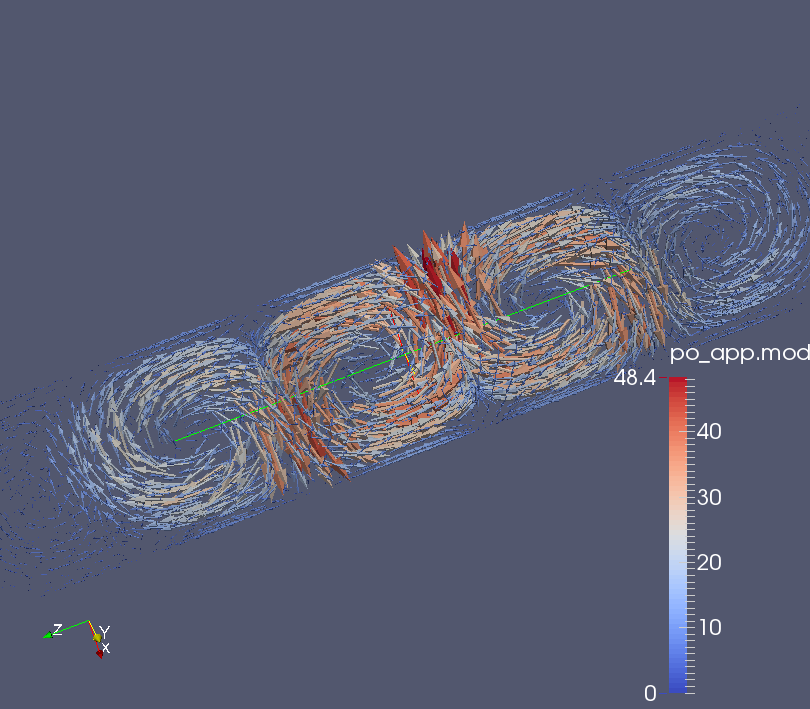
\includegraphics[scale=0.12]{glyphMode0}}\ 
		\subfloat[mode 5]{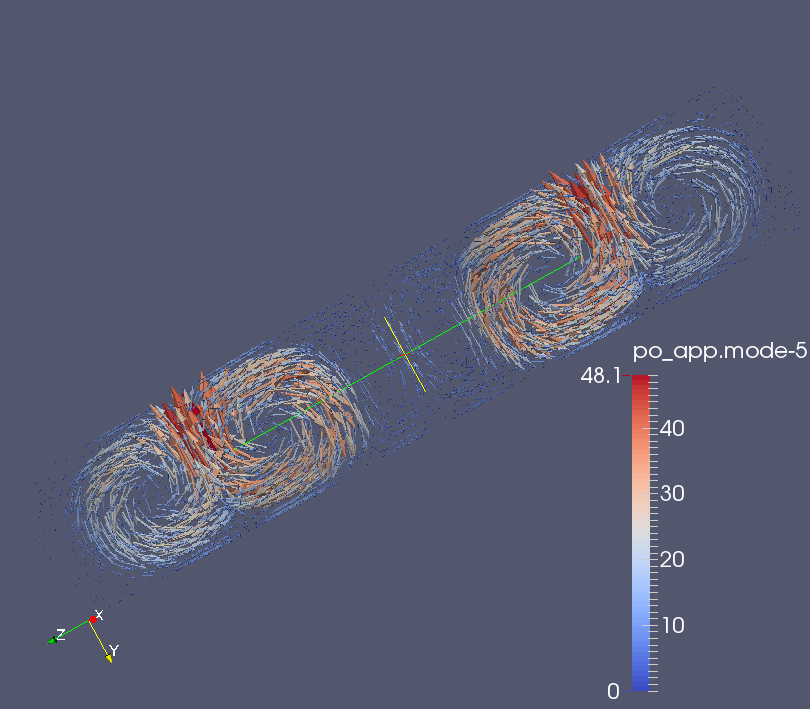
\includegraphics[scale=0.12]{glyphMode5}}
	}\\
	\makebox[\textwidth][c]{
		\subfloat[mode 10]{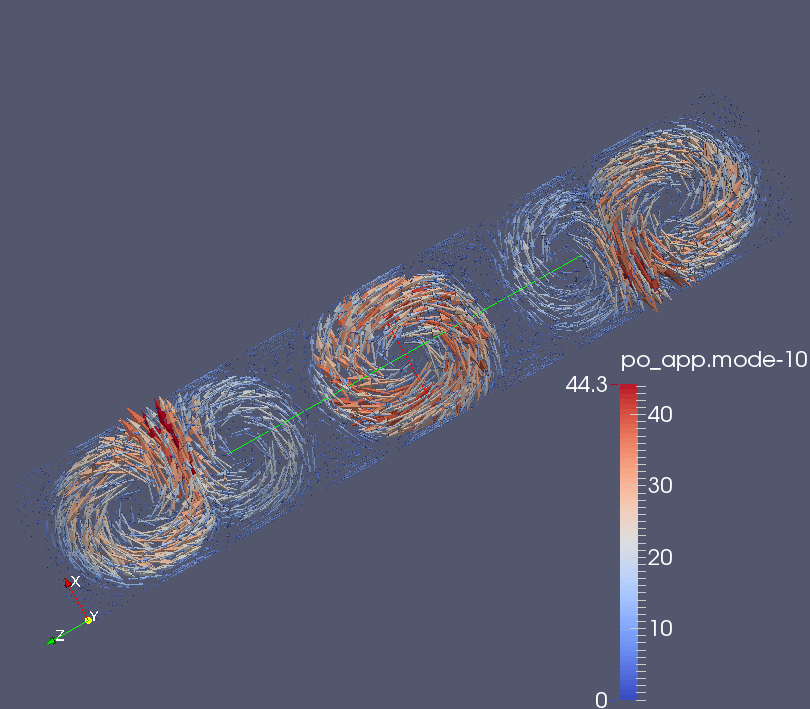
\includegraphics[scale=0.12]{glyphMode10}}\ 
		\subfloat[mode 14]{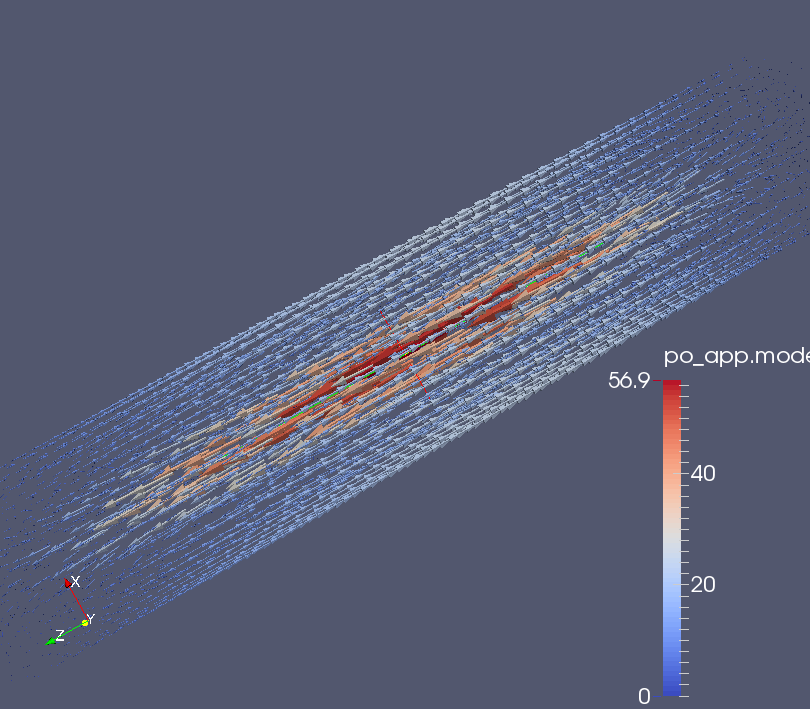
\includegraphics[scale=0.12]{glyphMode14}}
	}
	\caption{Modes propres}
	\label{resultats}
\end{figure}
\end{frame}

\begin{frame}{Problème spectral}
On observe que $\int_\Omega g^z = 0$, d'où, avec $\bm{f}=(0,0,9.81)$, on a
\[
R_{fk}=\int_\Omega \bm{f}\cdot\bm{g}=0
\]

De plus, $R_{pk}=\int_{\partial\Omega} \alpha_2\psi_k$, donc si $\psi$ est de moyenne nulle,
\[
R_{fk}=0
\]

On pose $\bm{c} = (c_0,c_1,\dots,c_M)$ et $A=\frac{\lambda^2}{Re}I+R_{iak}$, alors on résout
\[
Ac = R_{fk}+\frac{R_{pk}}{Re} = 0
\]
On cherche donc $\psi$ de moyenne non nulle.
\end{frame}

\end{document}
